\section{Objetivos}
\begin{itemize}
    \item Generar un patrón de interferencia utilizando un biprisma de Fresnel.
    \item Interpretar la estructura del patrón de interferencia en términos de la superposición de dos ondas.
    \item Determinar la longitud de onda de un láser a partir de la observación del patrón de interferencia y la geometría del montaje.
\end{itemize}

\section{Marco Teórico}
La luz se describe como un conjunto de perturbaciones eléctricas y magnéticas que se propagan a través del espacio, definidas por vectores de campo eléctrico y magnético que oscilan sincrónicamente. Cuando dos o más ondas coexisten en un mismo lugar, sus campos se suman vectorialmente, resultando en interferencia. Este fenómeno ocurre no solo en un punto, sino en una región donde las ondas coexisten, conocida como región de interferencia. El experimento de Young es una demostración clásica de interferencia donde un láser ilumina una pantalla con dos orificios, creando un patrón de franjas brillantes y oscuras en una pantalla de observación. Estas franjas resultan de la interferencia constructiva y destructiva de las ondas que emergen de los orificios.

\subsection{Interferencia Constructiva y Destructiva}
Ondas coherentes de la misma longitud de onda interfieren al superponerse. Si las ondas están en fase (diferencia de fase de cero o múltiplo de \(2\pi\)), interfieren constructivamente resultando en una amplitud combinada mayor y, por lo tanto, mayor intensidad. Si están en contrafase (diferencia de fase de \(\pi\) o un número impar de veces \(\pi\)), interfieren destructivamente, reduciendo o anulando la intensidad combinada.

\subsection{Localización de Franjas de Interferencia}
En el montaje de Young, la luz que incide en puntos específicos de la pantalla ha viajado a través de caminos de diferente longitud desde cada uno de los orificios, generando una diferencia de caminos que afecta la fase relativa de las ondas en esos puntos. Dependiendo de esta diferencia de caminos, las ondas pueden interferir constructiva o destructivamente, creando el patrón de franjas observado. La posición y separación de estas franjas se pueden predecir y analizar mediante principios geométricos y la relación de las longitudes de onda con las dimensiones del montaje.

\section{Montaje}
\textbf{Siguiendo las indicaciones de esta guía, realice el montaje.}

\section{Análisis y discusión: Determinación de la Longitud de Onda}

\subsection{Reporte de valores}
\textbf{Reporte los siguientes valores:}
\begin{itemize}
  \item Distancia focal $f$ de la lente: $0.02m$
  \item Distancia $f$ $+$ $A$ (entre la lente y el biprisma) medida: $0.02m + 0.047m$
  \item Valor de $A$ calculado: $0.047m$
\end{itemize}

\subsection{Reporte de valores $D$ y $L$}
\textbf{Reporte el valor medido de la distancia $D$ (entre el biprisma y la pantalla) y calcule $L$:}
\begin{itemize}
  \item $D$: $0.903$
  \item $L$: $0.93$
\end{itemize}

\subsection{Calcular separación entre fuentes}
\textbf{Asumiendo que $\alpha = 35\prime$ y que $n = 1.51$ , calcule la
separación $d$ entre las fuentes $S_{1}$ y $S_{2}$.}
\[ d = 2A\alpha(n-1) \]
\[ d = 0.000488081 \]

\subsection{$\Delta$$y$}
\textbf{Determine $\Delta$$y$.}

\[ \Delta y = 0.00028 \]


\subsection{Longitud de onda del láser}
\textbf{Calcule la longitud de onda del láser, con base en los datos anteriores.}

\[ \Delta y = \frac{L}{d}\lambda \]
\[ \lambda = \frac{\Delta y\times d}{L} \]
\[ \lambda = 1.47E-07 \]

\subsection{Variantes de medidas}
\textbf{Cambie el valor de alguno de los parámetros siguientes: $D$, $A$ ó $f$; Determine nuevamente la longitud de onda:}

\begin{figure}[H]
  \centering
  \begin{subfigure}[b]{\textwidth}
      \centering
      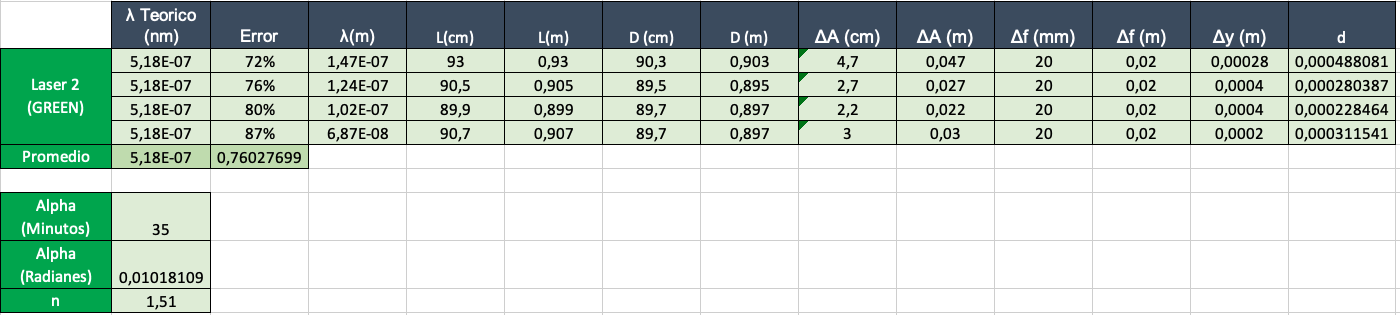
\includegraphics[width=\textwidth]{Figures/1. Content/tabla1.png}
      \caption{Tabla de diversos valores de longitud de onda}
      \label{fig: Diversos valores de longitud de onda}
  \end{subfigure}
  \hfill
\end{figure}

\subsection{Calculo de errores}
\textbf{Asuma $\lambda = 518nm$ como el valor teórico de la longitud de onda del láser de diodo
y calcule los porcentajes de error de las longitudes de onda obtenidas
experimentalmente.}

\begin{figure}[H]
  \centering
  \begin{subfigure}[b]{\textwidth}
      \centering
      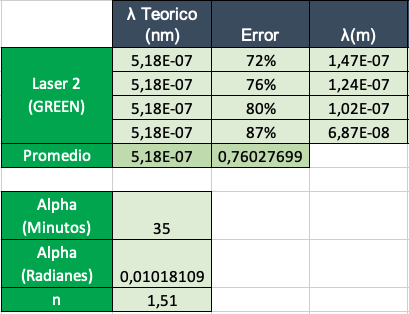
\includegraphics[width=0.4\textwidth]{Figures/1. Content/tabla2.png}
      \caption{Tabla de diversos porcentajes de error para cada longitud de onda}
      \label{fig: Tabla de diversos porcentajes de error para cada longitud de onda}
  \end{subfigure}
  \hfill
\end{figure}


\section{Causas de Error}
Las causas de error en este experimento sobre interferencia y el Experimento de Young podrían incluir:

\begin{itemize}
    \item \textbf{Alineación del sistema óptico:} Pequeños desajustes en la alineación de la lente y el biprisma pueden causar grandes desviaciones en los patrones de interferencia observados, afectando la precisión de las mediciones de la longitud de onda.
    \item \textbf{Calibración del equipo:} Errores en la calibración de los instrumentos de medición como el flexómetro y el pie de rey pueden introducir inexactitudes en las mediciones de distancias, afectando los cálculos de longitud de onda.
    \item \textbf{Estabilidad del láser:} Variaciones en la intensidad del láser debido a fluctuaciones en la alimentación eléctrica o condiciones ambientales como la temperatura pueden alterar la coherencia de la luz y, por ende, el patrón de interferencia.
    \item \textbf{Presencia de vibraciones:} Vibraciones en el ambiente de laboratorio pueden desplazar el equipo óptico durante la toma de datos, resultando en variaciones en la posición de las franjas de interferencia.
    \item \textbf{Difracción adicional:} Imperfecciones en los bordes del biprisma o suciedad en las superficies ópticas pueden introducir efectos de difracción adicionales que modifican el patrón de interferencia.
\end{itemize}

\section{Conclusiones}
Basado en los experimentos realizados, se concluye que:
\begin{itemize}
    \item \textbf{Confirmación del fenómeno de interferencia:} Los resultados experimentales confirmaron la teoría ondulatoria de la luz, mostrando patrones de interferencia consistentes con la interferencia constructiva y destructiva.
    \item \textbf{Medición de la longitud de onda:} Se logró determinar la longitud de onda del láser con una precisión razonable, utilizando la geometría del montaje y el patrón de interferencia. Los valores obtenidos estuvieron en general acuerdo con los valores teóricos esperados, aunque con variaciones que pueden atribuirse a las causas de error identificadas.
    \item \textbf{Importancia de la precisión experimental:} Este experimento resaltó la importancia de una cuidadosa configuración experimental y precisión en la medición para obtener resultados fiables en experimentos de óptica.
    \item \textbf{Educación práctica en óptica física:} La realización del experimento proporcionó una experiencia práctica valiosa en la manipulación y medición de fenómenos ópticos, reforzando la comprensión teórica y práctica de la interferencia de la luz.
    \item \textbf{Recomendaciones para futuros experimentos:} Se recomienda mejorar la estabilidad del montaje, realizar una calibración más exhaustiva de los instrumentos de medición y asegurar la limpieza completa de todas las superficies ópticas antes de realizar el experimento.
\end{itemize}
